\documentclass[journal]{IEEEtran}
%\documentclass[conference]{IEEEtran}
\IEEEoverridecommandlockouts
% The preceding line is only needed to identify funding in the first footnote. If that is unneeded, please comment it out.

\usepackage{url}
\usepackage{xspace}

\usepackage[Algorithm]{algorithm}
\usepackage{algorithmic}
\usepackage{setspace}

\usepackage{cite}
\usepackage{amsmath,amssymb,amsfonts}
\usepackage{algorithmic}
\usepackage{graphicx}
\usepackage{textcomp}
\usepackage{xcolor}
\usepackage{tabularx}

\usepackage{multirow}
\usepackage{booktabs}

\usepackage[spanish]{babel}
\usepackage[utf8]{inputenc}



%paquete para mostrar código
\usepackage{listings}
\usepackage{caption}
\lstset{
	basicstyle=\ttfamily\scriptsize, 
	columns=fullflexible, 
	%numbers=left, 
	%numberstyle=\tiny, 
	%numbersep=5pt,
	framexleftmargin=15pt,
	%framexrightmargin=17pt,
	framexbottommargin=2pt,
	framextopmargin=2pt,
	xleftmargin=15pt,
	frame=top,frame=bottom,
	captionpos=t,
	}

\captionsetup[lstlisting]{singlelinecheck=false, margin=0pt, labelsep=space,labelfont=bf}

%necesario para que diga Listado y no Listing	
\renewcommand{\lstlistingname}{Listado}	

\lstnewenvironment{sflisting}[1][]
{\lstset{#1}}{}

%%ejemplo de estilo para el lenguaje SPARQL

\lstdefinelanguage{sparql}{
	morecomment=[l][\color{teal}]{\#},
	morestring=[b][\color{blue}]\",
	morekeywords={SELECT,CONSTRUCT,DESCRIBE,ASK,WHERE,FROM,NAMED,PREFIX,BASE,OPTIONAL,FILTER,GRAPH,LIMIT,OFFSET,SERVICE,UNION,EXISTS,NOT,BINDINGS,MINUS,a,as,GROUP,BY,SUM,AVG,VALUES},
	sensitive=false
}

%listings styles
\lstdefinestyle{sparql}{
	basicstyle=\ttfamily\scriptsize, 
	language=sparql,
	columns=fullflexible, 
	numberstyle= \tiny, %\scriptsize,
	numbers=left,
	frame=lines,
	tabsize=2}

\lstdefinestyle{python}{
	basicstyle=\ttfamily\scriptsize, 
	language=Python,
	columns=fullflexible, 
	numberstyle= \tiny, %\scriptsize,
	%numbers=left,
	frame=lines,
	tabsize=2}


\makeatletter
\newcommand{\linebreakand}{%
\end{@IEEEauthorhalign}
\hfill\mbox{}\par
\mbox{}\hfill\begin{@IEEEauthorhalign}
}
\makeatother


\def\BibTeX{{\rm B\kern-.05em{\sc i\kern-.025em b}\kern-.08em
    T\kern-.1667em\lower.7ex\hbox{E}\kern-.125emX}}
\begin{document}

\title{GraFIng: Base de datos de grafos de la Facultad de Ingeniería de la Universidad de la República}


\author{
	\begin{tabular}{cc}
		\begin{tabular}{c}
			Graciana Castro                                              \\
			\textit{Facultad de Ingeniería, Universidad de la República} \\
			Montevideo, Uruguay                                          \\
			gcastro@fing.edu.uy
		\end{tabular}
		 &
		\begin{tabular}{c}
			Julian O'Flaherty                                            \\
			\textit{Facultad de Ingeniería, Universidad de la República} \\
			Montevideo, Uruguay                                          \\
			julian.o.flaherty@fing.edu.uy
		\end{tabular}
	\end{tabular}
}


\maketitle

\begin{abstract}
	El objetivo de este proyecto fue el diseño e implementación de una base de datos de grafos con información sobre individuos de la Facultad de Ingeniería de la Universidad de la República, Uruguay, y sus distintos trabajos. La información fue obtenida mediante \textit{scraping} de los sitios Colibrí\footnote{\url{https://www.colibri.udelar.edu.uy/jspui/}}, el repositorio institucional de la Universidad, y OpenAlex\footnote{\url{https://openalex.org/}}. Se implementó un grafo de propiedades y las consultas se realizaron utilizando \textit{Cypher}. Como resultado, se construyó una base de datos flexible que permite analizar relaciones entre autores y trabajos, facilitando consultas complejas y la visualización de la información académica de la institución.
\end{abstract}

\section{Introducción}
\label{introduccion}
El análisis de la producción científica y las redes de colaboración académica es una tarea de creciente importancia para las instituciones de investigación. La capacidad de identificar patrones de coautoría, seguir la evolución de líneas de investigación o descubrir conexiones interdisciplinarias aporta valor estratégico a la institución y fortalece a la comunidad científica. Sin embargo, la información académica suele encontrarse dispersa en múltiples repositorios, dificultando una visión integrada. Las bases de datos de grafos ofrecen una estructura adecuada para este desafío, ya que modelan de forma nativa las relaciones entre entidades como autores, publicaciones e instituciones, facilitando consultas que resultan inherentemente complejas en modelos de datos tradicionales.

En este contexto, el objetivo de este proyecto fue el diseño e implementación de una base de datos de grafos para centralizar y estructurar la información sobre los individuos y sus trabajos académicos en la Facultad de Ingeniería (Fing) de la Universidad de la República (UdelaR). Se buscó construir una herramienta que permitiera a investigadores, estudiantes y administradores analizar las redes de conocimiento de la institución de manera ágil e intuitiva.

Por tratarse de un trabajo de fin de curso, el alcance del proyecto se acotó a un subconjunto representativo y manejable del universo de datos. La población de estudio se limitó a los individuos (docentes y estudiantes) afiliados a tres institutos de la Fing: el Instituto de Ingeniería Eléctrica (IIE), el Instituto de Matemática y Estadística Rafael Laguardia (IMERL) y el Instituto de Computación (INCO) con trabajos publicados en Colibrí. Para ampliar y validar la información, se utilizó como fuente secundaria OpenAlex.

Este artículo detalla el proceso de construcción de dicha base de datos, desde la extracción de datos hasta la implementación del modelo de grafo, y demuestra su utilidad a través de ejemplos de consulta y análisis. El trabajo se organiza de la siguiente manera: la sección \ref{relacionados} revisa los antecedentes; la sección \ref{desarrollo} describe la metodología de diseño e implementación; la sección \ref{expe} presenta los resultados obtenidos, y finalmente, la sección \ref{conclusion} expone las conclusiones y líneas de trabajo futuro.

\section{Trabajos Relacionados}
\label{relacionados}
Existen antecedentes en el modelado de información académica mediante grafos, como la \textit{dblp computer science bibliography}\footnote{\url{https://dblp.org/}}, una base de datos de publicaciones del área de la informática que estructura la información en un grafo RDF. Su enfoque sirvió como modelo conceptual para nuestro sistema. Una inspiración directa fue el trabajo de fin de curso "El número Abreu" \cite{abreu2023}, realizado en 2023 para la asignatura Bases de Datos no Relacionales, que implementa la exploración de redes de jugadores de futbol y motivó la ejecución de una red similar para la comunidad académica de la Fing.

\section{Parte central}
\label{desarrollo}
En esta sección se describe el proceso de diseño e implementación de la base de datos de grafos, detallando las decisiones tomadas y los pasos seguidos.

\subsection{Obtención y Preprocesamiento de Datos}
El primer paso del proyecto fue la recolección de datos. Para ello, se desarrollaron herramientas de extracción automatizada (\textit{scraping}) en Python, organizadas en el módulo \texttt{udelar\_graph/extraction}. Las fuentes utilizadas fueron Colibrí y OpenAlex.

Para Colibrí, se implementó un extractor que recorría las páginas del repositorio, identificaba los registros relevantes y descargaba sus metadatos en formato XML. Posteriormente, estos archivos fueron procesados para extraer información estructurada como autores, títulos y afiliaciones. Este procesamiento incluyó tareas de normalización y deduplicación de registros.

En paralelo, se utilizó la API pública de OpenAlex para enriquecer los datos locales con identificadores externos, temas y métricas de citación. La integración de los datos de ambas fuentes se realizó mediante la correspondencia de identificadores y la comparación de metadatos clave. Una vez procesados, los datos consolidados se almacenaron en archivos estructurados (JSON y XML) en la carpeta \texttt{data/}, listos para su carga en el grafo. Este preprocesamiento resultó esencial para asegurar la calidad y coherencia de la información.

\subsection{Modelado y Carga del Grafo}
Para el modelado se optó por un grafo de propiedades, gestionado con la base de datos Neo4j. En este modelo, los nodos representan entidades (Personas, Trabajos, Tipos de Trabajo y Palabras Clave) y las relaciones modelan los vínculos entre ellas (autoría, contribución, tipo y palabra clave). La Figura~\ref{fig:grafo} ilustra el esquema del grafo implementado.

\begin{figure}[h]
	\centering
	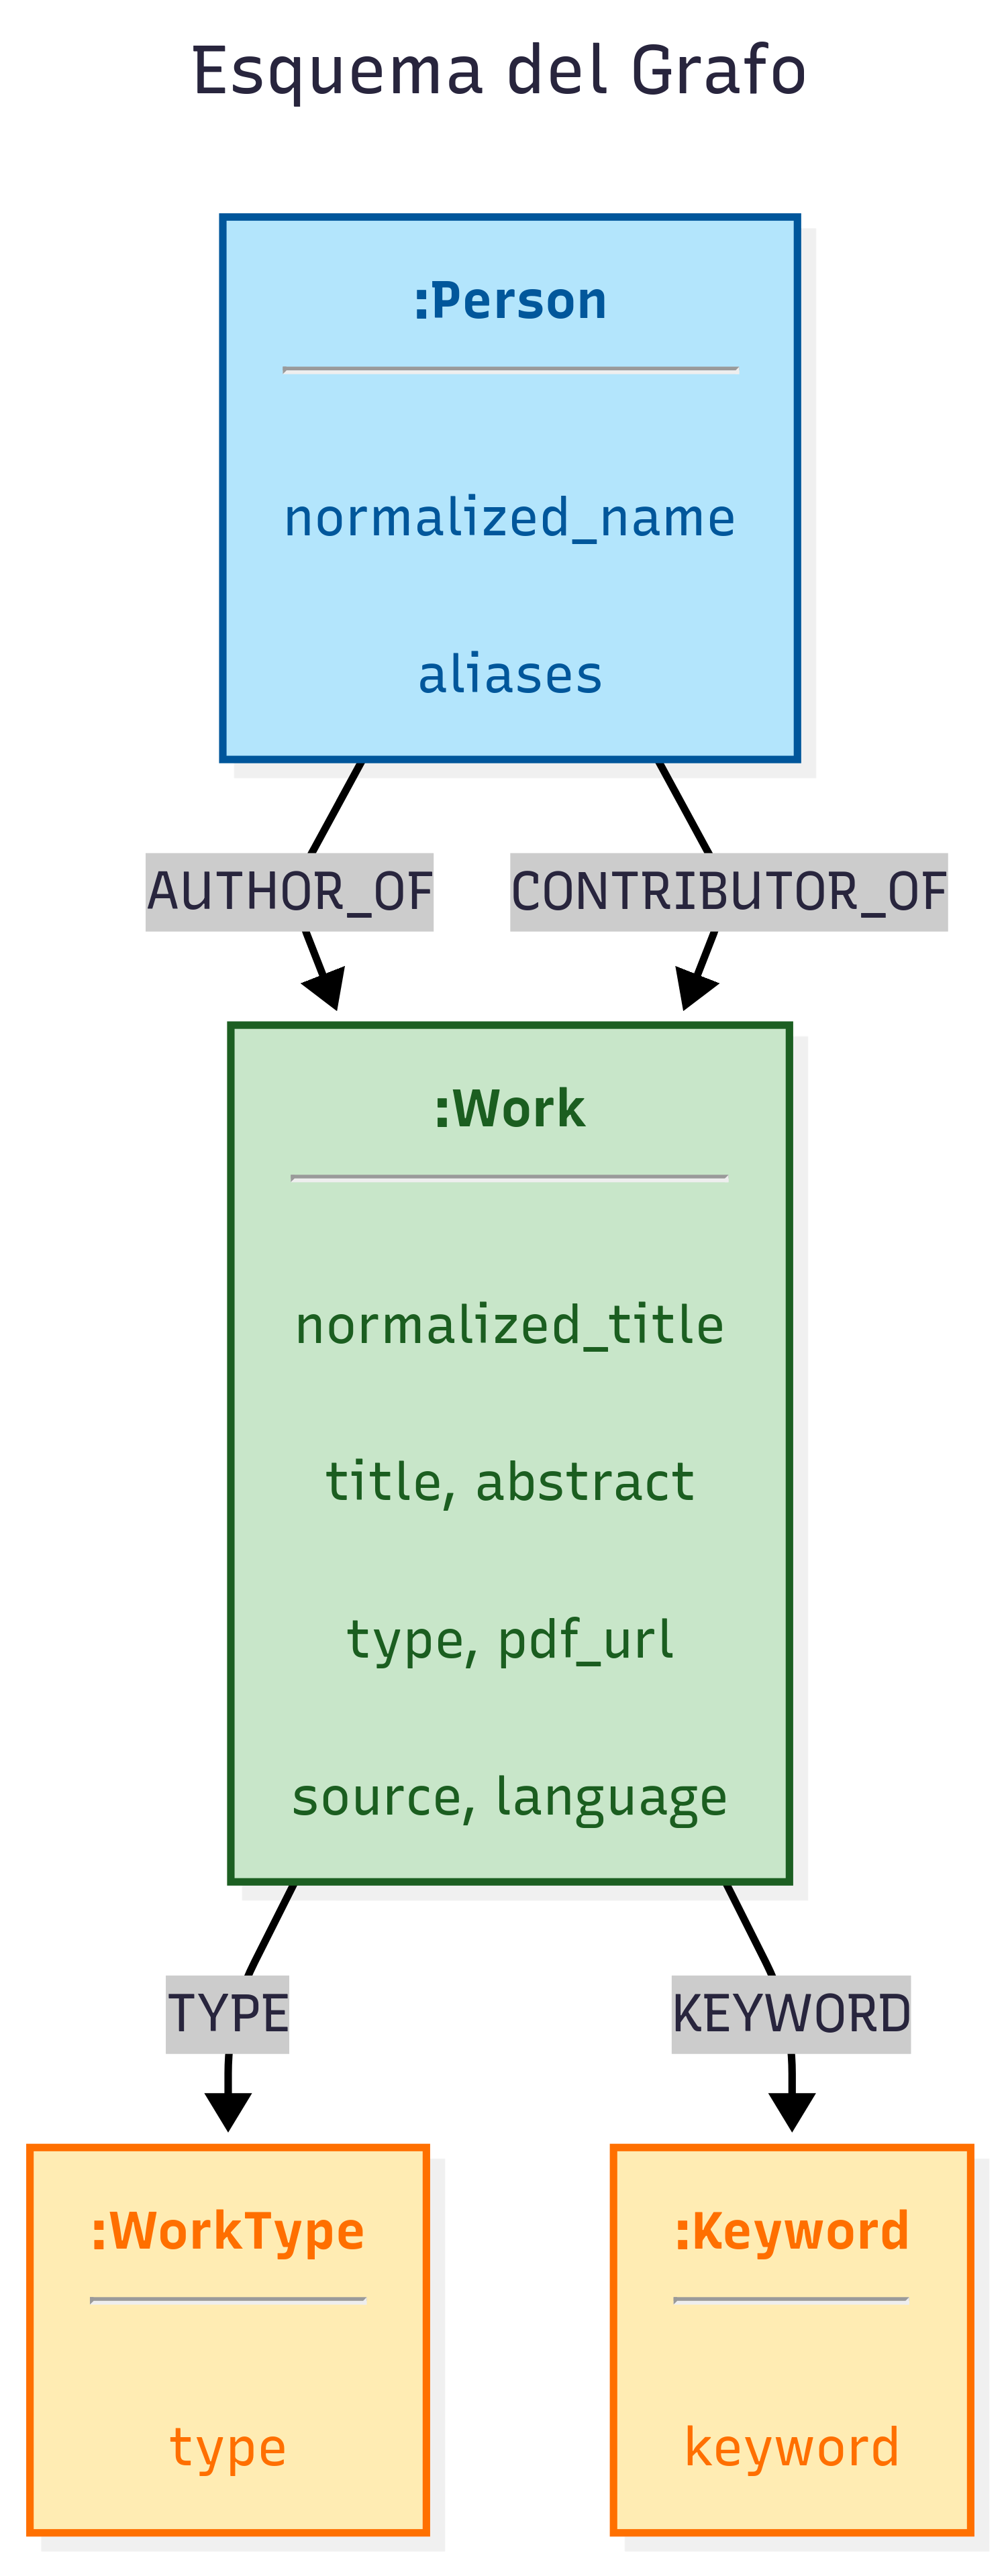
\includegraphics[width=0.6\linewidth]{imagenes/grafo.png}
	\caption{Esquema del grafo de propiedades implementado.}
	\label{fig:grafo}
\end{figure}

La carga de los datos se automatizó mediante scripts de Python que utilizan la biblioteca oficial de Neo4j. El proceso, encapsulado en el módulo \texttt{udelar\_graph/load/colibri.py}, transforma los datos preprocesados en nodos y relaciones mediante consultas Cypher. Para facilitar la ejecución, se implementó una interfaz de línea de comandos (CLI) con la biblioteca Typer. El comando \texttt{colibri-load} permite poblar la base de datos, incluyendo una opción para limpiarla previamente y así garantizar la reproducibilidad de los experimentos. Una vez cargados los datos de Colibrí, se ejecutó el comando \texttt{openalex-load} para integrar los datos de OpenAlex.

\subsection{Limitaciones}
El desarrollo del sistema enfrentó limitaciones inherentes a las fuentes de datos y al alcance del proyecto. La cobertura de Colibrí no es exhaustiva y presenta inconsistencias en sus metadatos. Aunque la integración con OpenAlex mitigó parcialmente este problema, la correspondencia entre registros no siempre fue directa. Por otra parte, el estudio se restringió a tres institutos de la Facultad, lo que limita la representatividad del grafo resultante. Finalmente, la implementación se realizó sobre una instancia local de Neo4j, con las consiguientes restricciones de escalabilidad. Estas limitaciones abren claras oportunidades para trabajo futuro, como la ampliación del conjunto de datos y la mejora de los procesos de limpieza y normalización.

\section{Experimentación}
\label{expe}

\subsection{Consultas}
Para validar la utilidad del grafo, se diseñaron y ejecutaron diversas consultas en Cypher que responden a preguntas de interés académico. A continuación, se presentan algunos ejemplos representativos.
%(Aquí se pueden incluir listados de código Cypher y los resultados obtenidos, ya sea en tablas o con visualizaciones).

\section{Conclusiones y Trabajo Futuro}
\label{conclusion}
Este proyecto demostró que el modelado de la producción académica de la Facultad de Ingeniería en una base de datos de grafos es una aproximación factible y potente. La integración de fuentes como Colibrí y OpenAlex en un único grafo resultó ser una solución eficaz para centralizar y conectar información, mientras que el uso del lenguaje de consulta \textit{Cypher} otorgó una gran flexibilidad para explorar relaciones complejas, como patrones de coautoría y vínculos temáticos, de una manera ágil e intuitiva.

El trabajo en su conjunto constituye una sólida prueba de concepto. Aunque el estudio se limitó a tres institutos, la arquitectura del sistema está diseñada para crecer. Posibles líneas de trabajo futuro son: expandir el grafo para incluir a todos los investigadores de la Facultad, e incorporar nuevas entidades como filiación para identificar colaboraciones interinstitucionales. Estos pasos permitirían transformar el prototipo actual en un recurso analítico de gran valor estratégico para la institución.

%\bibliographystyle{plainnat}
\bibliographystyle{IEEEtran}
\bibliography{final-article}


\end{document}